\chapter{考察}
本章では,その性能や回路スケールに影響を及ぼす要因や
遅延時間以外の設計選択肢について考察していく.
\section{遅延時間差の検知}
光Race Logic回路を構成するためには,
光伝搬信号に遅延時間を重みとして付加していくarray部分だけではなく
遅延時間差を検知する部分が必要となる.
これを検知部分と呼称する.

本提案の光Race Logic arrayは図\ref{fig:scorematrix_3}に示すスコアマトリクスを使用している.
この場合には,光伝搬出力信号の時間差は一つのセルの通過時間単位で変化する.
よって,検知部分では一つのセルの通過時間の差を検知できれば良い.
ゲート長が1$\mu m$の場合,一つのセルの通過時間は12.52psである.
デジタルカウンタを用いて遅延時間差を検知部分を構成すると,カウンタを約80GHzで動作させなければならない.

また,使用するスコアマトリクスを変化させた場合も考える.
図\ref{fig:scorematrix_4}にスコアマトリクスの一例を示す.
\begin{figure}[t!]
\begin{center}
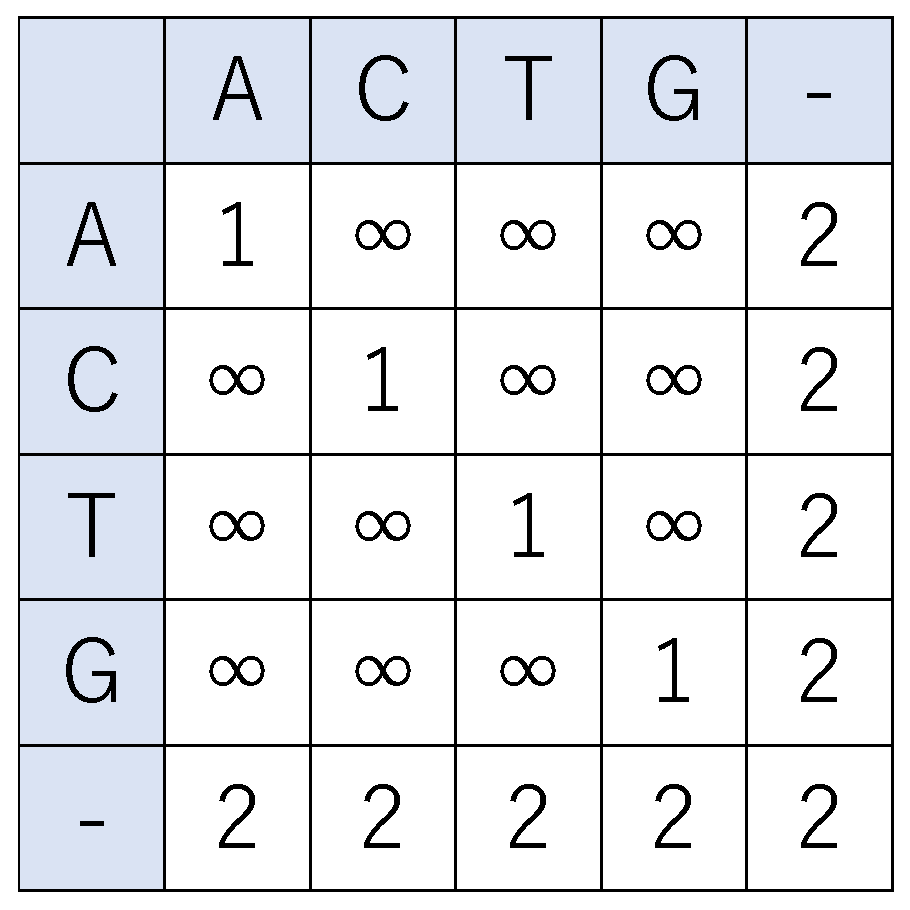
\includegraphics[keepaspectratio,scale=0.4]{fig/5/scorematrix_4.eps}
\caption{スコアマトリクスの一例}
\label{fig:scorematrix_4}
\end{center}
\end{figure}
このスコアマトリクスでは,図\ref{fig:scorematrix_3}に示すスコアマトリクス
とは違い,欠損・挿入に対応するギャップスコアが2となっている.
本提案の光Race Logic arrayでは,光遅延素子で発生させる遅延時間を
光スイッチを通過する際の遅延時間の倍とすることで図\ref{fig:scorematrix_4}に示す
スコアマトリクスに基づく配列アラインメントスコアを求めることができる.
この場合,光伝搬出力信号の時間差は光スイッチの通過時間単位で変化し,
光スイッチの通過時間はそのゲート長にて決定される.
ゲート長の最小加工寸法が1$\mu m$である時,
光スイッチを通過する際の遅延時間は10$fs$であり,光遅延素子にて発生させる遅延時間は
20$fs$である.
検知部分では10$fs$の遅延時間差を検知できなければならない.
もしデジタルカウンタを用いて遅延時間差を検知部分を構成する仮定すると,
カウンタを100THzで動作させなければならない.

その様な動作周波数でデジタルカウンタを動作させることは不可能である.
よって,検知部分をデジタルカウンタで構成した場合には,
検知部分が光Race Logic回路の性能を律速する要因となる.

光Race Logic arrayをもって光伝搬信号の遅延時間に情報を付与できることは
本研究の検証によって明らかになった.
この光Race Logic arrayの光速での計算能力を活かす
検知部分の構成を考えることが必要である.

\section{雑音の影響}
\subsection{光伝搬信号強度に影響を与える雑音}
検出可能な強度を担保する必要がある
光伝搬信号の特徴
雑音が素子を通るたびに蓄積していく
Nのスケーリングに影響を及ぼす
\subsection{遅延時間に影響を与える雑音}
製造ばらつきが要因になるものに代表される
素子の伝搬遅延誤差
伝搬遅延の誤差も素子を通るたびに蓄積
とある配列の組み合わせにおいて想定される遅延時間と
実際の出力の遅延時間に差が生じる
製造ばらつきであればある程度チューニングが可能か?
スコア1の重みをどの程度の遅延時間と定めるかによって
Nのスケーリングに影響を及ぼす.

\section{遅延時間以外の設計選択肢}
